\section{Results}
\label{sec:res}
In this section, we will discuss the results obtained by classification and word-pair difficulty ranking, 
%including the performance on various features and comparisons between baseline models and our feature engineering model.
including the comparisons between baseline models and our multi-faceted features model and the ablation tests for feature selection.

\subsection{Baseline Models}
In this section, we introduce the design of baseline models for the contrast experiments on classification and word-pair ranking tasks.
\subsubsection{Human Baseline}
To observe the limitation of human on classifying the word difficulty levels, 5 experts with educational background in foreign languages are chosen to do the classification task and word-pair difficulty ranking task respectively.
For classification task, each person was pre-trained with several words randomly selected from the standard difficulty levels, and were asked to allocate the difficulty levels for  100 words according to their learning outcomes and previous knowledge.
%In order to follow the actual distribution of word levels, the words to be labeled have the same distribution.
For difficulty ranking task, each person was given 100 pairs of words to label the difficulty relation of each pair. 
The words to classify and the word pairs are randomly sampled from the word list with the same distribution.
%Then we calculate the inter-judge agreement using Cohen's Kappa measurement. 

\subsubsection{Random Baseline (Random)}
In classification task, we follow the original distribution of word levels and randomly assign a level for each word and calculate the average accuracy of 10 runs.
In difficulty ranking task, 
each word pair will be randomly assigned with a difficulty relation.
%each word will be randomly assigned with a word in difficulty level to make up a word pair.
Then the accuracy will be calculated as the average of 10 runs.

\subsubsection{Frequency-Only Baseline (FO)}
%Frequency is a means of estimating the word difficulty. 
%As mentioned before, word difficulty has negative correlation with its frequency.
Frequency is a considerable feature on estimating the word difficulty.
%Some research discussed the correlation between word frequency and word difficulty, finding they are highly correlated~\cite{breland1996word}.
%There also exist some websites estimating the word difficulty based on word frequency\footnote{\url{https://www.twinword.com/api/language-scoring.php}}.
To construct the frequency-only baseline model, 
we calculate the word frequencies 
%of an open frequency dataset and a single corpus used in our experiment.
%\textbf{Frequency-only model based on the open dataset (FOMO)} calculates the English words' frequencies from SUBTLEX-UK list~\cite{van2014subtlex} and the  German words' frequencies from SUBTLEX-DE list~\cite{Bryant2011}.
%\textbf{Frequency-only model based on single corpus (FOMS)} calculates word frequencies 
based on different $Corpus$ mentioned in Section \ref{sec:data}.
The approach to construct the dataset for both classification and ranking tasks are the same as previous. 

%The open frequency list here means the SUBTLEX-UK list~\cite{van2014subtlex} for English or SUBTLEX-DE list~\cite{Bryant2011} for German.
%The words of SUBTLEX lists are both collected from subtitles of television programs, ordered by their frequencies.
%The single corpus used in our experiment is E1, E2 or G1 mentioned in Section \ref{sec:exper}.

\subsubsection{Frequency-Clustering Baseline (FC)}
Xiaobin Chen \shortcite{chen2016characterizing} implemented text readability classification by calculating mean frequencies of words from vocabulary bands and clusters respectively.
In this paper, we apply the clustering method to divide the vocabulary frequency bands.
%Intuitively, the distance between two words is the difference between their frequencies, so k-means is used for cluster analysis.
Intuitively, the Euclidean distance between each two words can be regarded as the difference on their frequencies:
$dist(w_i, w_j)=|Freq_{w_i}-Freq_{w_j}|$, then
we use K-means to do the clustering.
%As expected, the results of the cluster are consistent with the word frequencies distribution.
%The results of the clustering are consistent with the frequency distribution of words.
%The clustering results on The New York Times (E1) are shown as Figure \ref{fig:cluster}.
%It's clear that the frequencies bands can be  obviously divided by clustering.
Similarly, this baseline is also implemented on different $Corpus$ and different tasks.
%\SY{reviewer 2: There is no obvious clustering here.}

%\begin{figure}[th]
%	\centering
%	%	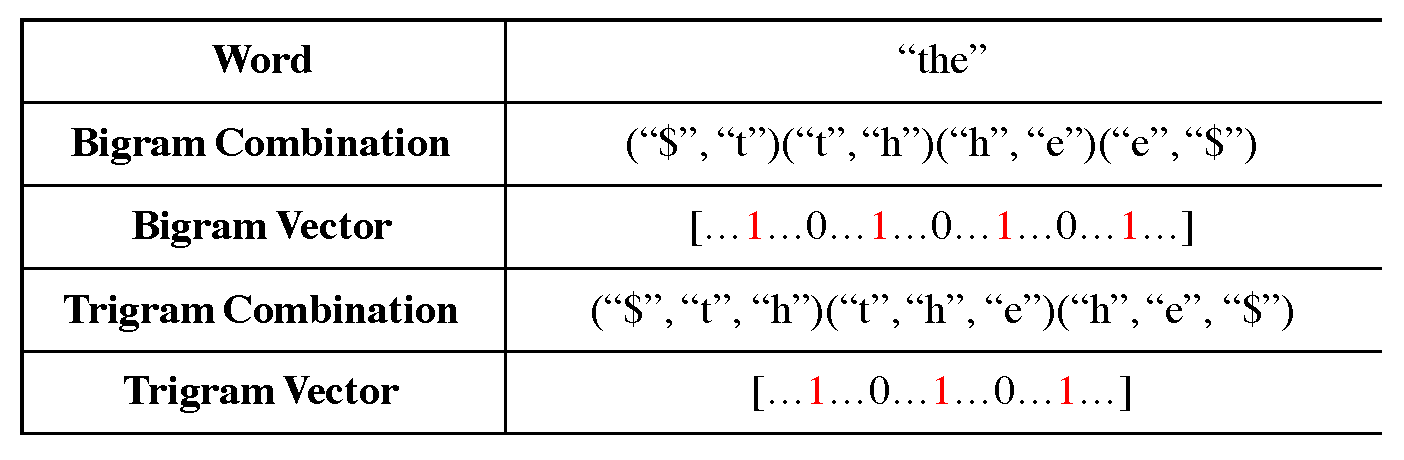
\epsfig{file=pic/bitri.eps, width=0.9\columnwidth}
%	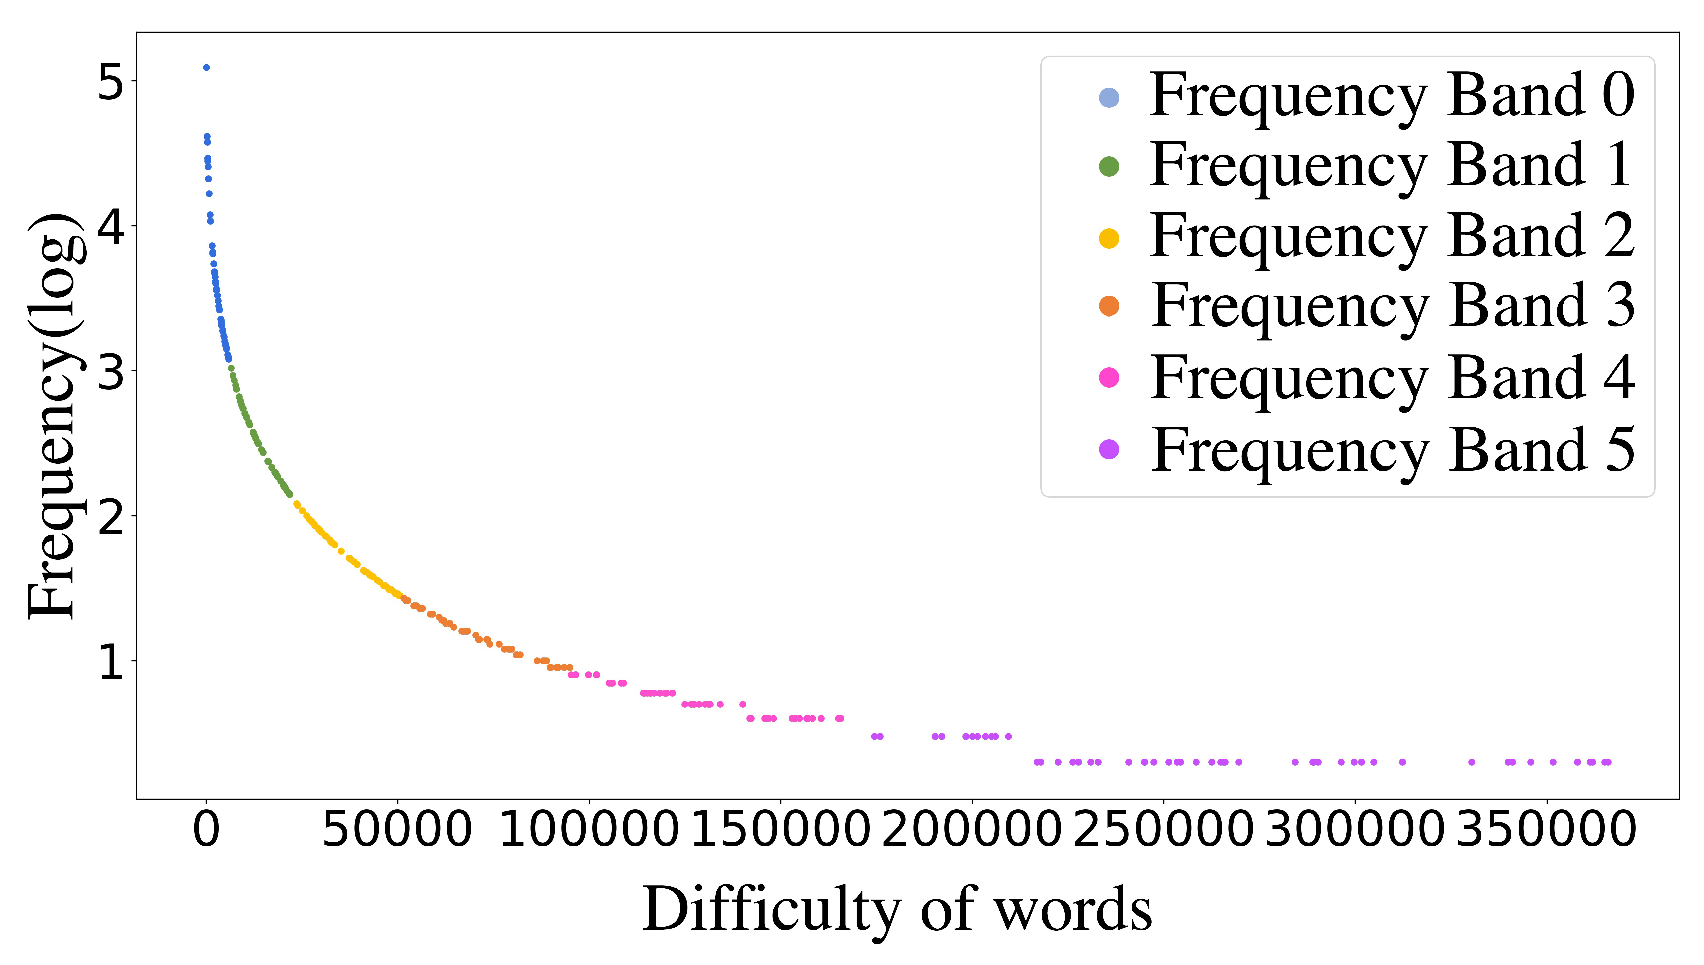
\includegraphics[width=1\linewidth]{pic/cluster.eps} 
%	\caption{Frequencies bands divided by clustering of the New York Times. The horizontal axis is the ranking of words ordered by difficulty, and the vertical axis is the log value of frequency.}
%	\label{fig:cluster}
%\end{figure}

%\textbf{FC Model based on the open frequency datasets (FCMO)} is implemented on English and German SUBTLEX lists.

%\textbf{FC Model based on the single corpus (FCMS)} is implemented on E1, E2 and G1 respectively.

%However, it can only achieve the accuracy of 8.91  of in English and the accuracy of 30.14  in German by predicting the word difficulty level by dividing the frequency of words into words.
%Once again proved that the difficulty of some words is not estimated completely by its frequency.
\subsubsection{Multi-Features Baseline}
%Several related studies in the fields of education and linguistics have mentioned that the compound of word frequency, length, the number of syllables in a word and the number of consonant clusters in a word~\cite{koirala2015word} and the compound of word frequency and POS tag~\cite{hiebert2019analysis} can be the features to measure word difficulty.
Several related studies in the field of education and linguistics combine features to do their tasks. 
The combination of frequency, length, syllables and phonemes and the number of consonant clusters is used in Koirala and Culligan's work~\shortcite{koirala2015word,culligan2015comparison}. 
Hiebert et al.~\shortcite{hiebert2019analysis} used word frequency and POS tags together to measure word difficulty.
Following these studies, we conduct the \textbf{FLSCP} (Freq+Length+\#Syllables+\#Consonant+\#Phonemes) baseline and \textbf{FPOS} (Frequency+POS) baseline.
%We also build \textbf{FLSCPV} (Freq+Length+\#Syllables+\#Consonant+Phoneme Binary Vector) which replaces the number of phonemes with the phoneme binary indication vector mentioned in Section \ref{sec:approach} to give a more fair and comprehensive comparison. 
Since these studies are only theoretical research and lack of automatic classification experiments, 
we use MLP to do the classification and ranking tasks based on these compound features.

\subsection{Results for Multi-faceted Features}
\label{sec:mmf}
%In this part, we discuss the results of our feature engineering method and other baseline models.
%The experiment is conducted on E1, E2, E1+E2 and G1.
%According to the result of the multi-class classification and difficulty ranking tasks shown in Table \ref{tab:resultsEnglish} and Table \ref{tab:resultsGerman}, we can draw the conclusion as follows.
The results of word difficulty classification and word-pair difficulty ranking tasks are shown in Table \ref{tab:resultsEnglish} and Table \ref{tab:resultsGerman} for different languages.
\textbf{MMF} represents the Multi-faceted Features mentioned in Section \ref{sec:approach}.
\begin{table*}[h]
	\scriptsize
	\setlength{\abovecaptionskip}{0pt}
	\setlength{\belowcaptionskip}{0pt}
	\begin{center}
		\begin{tabular}{lcccccccccccc}
			\toprule[1pt]
			& \multicolumn{4}{c}{\textbf{\begin{tabular}[c]{@{}c@{}}NY Times\end{tabular}}} & \multicolumn{4}{c}{\textbf{\begin{tabular}[c]{@{}c@{}} Gutenberg\end{tabular}}} & \multicolumn{4}{c}{\textbf{NY Times+Gutenberg}} \\ 
			\midrule
			& \multicolumn{2}{c}{\textbf{Classification}} & \multicolumn{2}{c}{\textbf{Ranking}} & \multicolumn{2}{c}{\textbf{Classification}} & \multicolumn{2}{c}{\textbf{Ranking}} & \multicolumn{2}{c}{\textbf{Classification}} & \multicolumn{2}{c}{\textbf{Ranking}} \\ 
			\midrule
			& \multicolumn{1}{c}{\textbf{Test}} & \multicolumn{1}{c}{\textbf{\textbf{CV}}} & \multicolumn{1}{c}{\textbf{Test}} & \multicolumn{1}{c}{\textbf{CV}} & \multicolumn{1}{c}{\textbf{Test}} & \multicolumn{1}{c}{\textbf{\textbf{\textbf{CV}}}} & \multicolumn{1}{c}{\textbf{Test}} & \multicolumn{1}{c}{\textbf{CV}} & \multicolumn{1}{c}{\textbf{Test}} & \multicolumn{1}{c}{\textbf{CV}} & \multicolumn{1}{c}{\textbf{Test}} & \multicolumn{1}{c}{\textbf{CV}} \\ 
			\midrule
			\textbf{Random}&20.57 &20.57 &49.85 &49.85 &20.57 &20.57 &49.85 &49.85 &20.57 &20.57 &49.85 &49.85 \\
			\textbf{FC}&8.23&8.23&67.50&67.50&17.53&17.53&30.36 &30.36 &22.41 &22.41 &55.00 &55.00 \\
			\textbf{FO}&34.20 &33.55 &66.10 &64.23&27.94&29.26&55.13 &57.56 &26.91 &28.23 &51.92 &53.22 \\
			\textbf{FPOS}&33.18&33.47&52.06&64.14&29.14&29.14&52.55&56.93&28.19&29.28&54.87&57.41 \\
			\textbf{FLSCP}&33.78&34.45&68.49&66.22&28.70&29.13&62.06&59.69&26.56&28.38&60.56&58.87\\
			\midrule
			%			[Fix+Word2Vec]+SVM&40.84 &39.59 &75.59 &78.77 &41.07 &36.36 &73.63 &74.31 &43.85 &39.32 &70.89 &65.74 \\
			\textbf{MFF+SVM$^{***}$}& 40.84& \textbf{39.59} & \textbf{75.59} & \textbf{78.77}& 41.07& \textbf{36.36} & 73.63 & \textbf{74.31} & \textbf{43.85} & \textbf{39.32}& 70.89& 65.74\\ 
			\textbf{MFF+MLP$^{***}$}&\textbf{42.94}&37.62&74.91&72.13&\textbf{41.18}&34.45&\textbf{74.88}&68.68&42.83&36.65&\textbf{76.29}&\textbf{72.76}\\
			%			[Fix+GloVe]+SVM&38.75 &36.56 &68.54 &65.43 &37.12 &36.25 &64.88 &62.05 &38.98 &36 &67.62 &63.48 \\
			%			[Fix+BERT]+SVM&41.76 &39.52 &74.15 &77.95 &42.46 &40.52 &73.5 &78.29 &43.85 &40.83 &71.93 &79.46 \\
%			\textbf{Fix+BERT}&42.11 &36.93 &68.55 &67.58 &\textbf{41.76 }&\textbf{35.78 }&64.19 &\textbf{69.12 }&\textbf{43.23 }&\textbf{38.92 }&65.48 &70.26 \\
%			\textbf{Fix+GloVe}&36.80 &34.97 &67.01 &67.35 &38.77 &34.86 &62.70 &68.22 &38.68 &35.15 &66.29 &69.72 \\
			\midrule
			\textbf{Human baseline}&49.28 &-&88.89 &-&49.28 &-&88.89 &-&49.28 &-&88.89 &-\\
			\bottomrule[1pt]
		\end{tabular}
	\end{center}
	\caption{\label{tab:resultsEnglish} 
		The classification and ranking results 
		%		 of different baseline models and our feature engineering methods by averaging ten runs 
		using two English $Corpus$ and their combination to extract the features.
		The accuracy for baseline models and our feature engineering models is the average of ten runs.
		\textbf{Test} means the accuracy on test set and \textbf{CV} means the accuracy on cross validation.
		\textbf{MFF} is the multi-faceted features using Word2Vec to obtain word embeddings.
		(*** indicates $p$-$value$ $<0.01$ compared with Random, FC, FO, FPOS and FLSCP baselines.)}
\end{table*}

\begin{table}[ht]
	\scriptsize
	\setlength{\abovecaptionskip}{0pt}
	\setlength{\belowcaptionskip}{0pt}
	\begin{center}
		\begin{tabular}{lcccccccc}
			\toprule[1pt]
			& \multicolumn{4}{c}{\textbf{\begin{tabular}[c]{@{}c@{}}Parallel Corpus for German\end{tabular}}} & \multicolumn{4}{c}{\textbf{\begin{tabular}[c]{@{}c@{}}Wikipedia for Chinese\end{tabular}}}\\ 
			\midrule
			& \multicolumn{2}{c}{\textbf{Classification}} & \multicolumn{2}{c}{\textbf{Ranking}} & \multicolumn{2}{c}{\textbf{Classification}} & \multicolumn{2}{c}{\textbf{Ranking}}\\ 
			\midrule
			& \multicolumn{1}{c}{\textbf{Test}} & \multicolumn{1}{c}{\textbf{CV}} & \multicolumn{1}{c}{\textbf{Test}} & \multicolumn{1}{c}{\textbf{CV}} & \multicolumn{1}{c}{\textbf{Test}} & \multicolumn{1}{c}{\textbf{CV}} & \multicolumn{1}{c}{\textbf{Test}} & \multicolumn{1}{c}{\textbf{CV}}\\ 
			\midrule
			\textbf{Random}&33.61 &33.61 &47.14 &47.14  & 16.63 &16.63 &43.03&43.03\\
			\textbf{FC}&34.93 &34.93 &49.24 &49.24 & 33.84 &33.84 &40.87	&40.87\\
			\textbf{FO}&36.83 &36.87 &53.42 &48.49 &54.02&	52.68&	62.99&	64.75\\
			\textbf{FPOS}&37.69 &36.77 &50.88 &48.44 &53.34	&53.17	&63.61	&65.90\\
			\textbf{FLSCP}&39.22 &37.46 &52.07 &53.67 &55.16&	53.77	&67.26	&66.60\\
			\midrule
			%			[Fix+Word2Vec]+SVM&42.39 &42.46 &70.47 &64.23 \\
			\textbf{MMF+SVM}&42.39$^{***}$	& 42.46$^{***}$ & \textbf{70.47$^{***}$}	& \textbf{64.23$^{***}$} & \textbf{57.80$^{***}$}	&54.95$^{***}$	&67.51$^{**}$	&\textbf{76.35$^{***}$}\\
			\textbf{MMF+MLP}&\textbf{47.74$^{***}$}&\textbf{42.50$^{***}$}&67.91$^{***}$ & 63.45$^{***}$  &56.96$^{***}$	&\textbf{55.84$^{***}$}	&\textbf{68.52$^{**}$}	&65.90$^{*}$\\
			%			[Fix+GloVe]+SVM &41.98 &42.42 &69.07 &65.74 \\
			%			[Fix+BERT]+SVM &42.39 &37.28 &52.88 &64.05 \\
%			\textbf{Fix+BERT}&46.30 &38.98 &54.14 &63.32 \\
%			\textbf{Fix+GloVe}&46.91 &41.73 &67.51 &69.14 \\
			\midrule
			\textbf{Human baseline}&44.44 &-&65.85 &-&&-&&-\\
			\bottomrule[1pt]
		\end{tabular}
	\end{center}
	\caption{\label{tab:resultsGerman} 
		The classification and ranking results using German and Chinese $Corpus$ to extract features.
		(*** indicates $p$-$value$ $<0.01$ compared with Random, FC, FO, FPOS and FLSCP baselines;
		** indicates $p$-$value$ $<0.01$ compared with Random, FC, FO and FPOS baselines;
		* indicates $p$-$value$ $<0.01$ compared with Random and FC baselines.)
%		The accuracy for baseline models and our feature engineering models is the average of ten runs.
%		\textbf{Test} means the accuracy on test set and \textbf{CV} means the accuracy on cross validation.
%		\textbf{Fix} is the compound features mentioned in this paper except word embedding.
		}
\end{table}
	
%	The explanation for this phenomenon is that FO focuses on word frequency itself and FC focuses on the frequency distribution of all words. 
%	There are more words in Gutenberg dataset which provides strong support to FC.
%	However a considerable part of words are older than those in New York Times, and this is the reason why it doesn't perform well on FOMS.

Comparing the results of baseline models for English such as FO, FC, FPOS, FLSCP and FLSCPV under NyTimes, Gutenberg and NyTimes+Gutenberg,
we find that the accuracy on both tasks varies substantially across different corpora.
%	Combined with the results in Section \ref{\textbf{sec:embedding}}, frequency is the best in the performance of the classification compared with length, POS and .
One possible explanation is that the large disparity in word frequency distribution leads to the unstable classification results among corpora. 
We found the P-value is less than 0.001 between the word frequency distribution of 
NyTimes and Gutenberg, which indicates there exists a significant difference.
%Thus, one possible explanation for the results is that the large disparity in word frequency distribution leads to the unstable classification results. 
Besides, 8 of the words in test set is correctly classified with features extracted under NyTimes while wrongly classified under Gutenberg and NyTimes+Gutenberg, which also supports the above conjecture.

Compared with the baselines, our proposed model takes more features 
into consideration, especially the syntactic and semantic features.
In Table \ref{tab:resultsEnglish}, we find that the results for both tasks are similar under different corpora and different classifiers, 
which are shown in the rows titled \textbf{MFF+SVM} and \textbf{MFF+MLP}.
The results in these two rows are significantly better than the baselines by T-test with $p$-$value$ $<0.01$.
Applied to different languages such as German and Chinese, the results of \textbf{MFF+SVM} and \textbf{MFF+MLP} in Table \ref{tab:resultsGerman} still have better performances than baselines.
Although frequency plays an important role in Chinese, the result also shows the superiority of multi-faceted features. 
The performance on three languages indicates that multi-faceted features 
is essential and effective for word difficulty classification.
It is also relatively stable among different language environments, showing a strong generalization ability which can 
be used in diverse language environments.
	
%Our proposed feature engineering model achieves the best results compared with previous models and it can achieve around 45  on classification task and 75  on ranking task.
%Overall, all the compound features with various embeddings on different corpus environments have shown to be significantly better than the previous state-of-the-art methods by T-test with p$<$0.01.

%From some prediction results of FO and ALL in Table \ref{tab:com}, we find our model can put some easy words into the correct level.
%Considering the words that are wrongly predicted by FO while correctly predicted by Fix+Word2Vec, Table \ref{tab:com} lists some examples to show our model is more inclined to classify the easier ones correctly.
%\begin{table}[th]
%	\scriptsize
%	\begin{center}
%		\begin{tabular}{ccccc}
%			\hline
%			\textbf{Word} & \textbf{Frequency in E1} & \textbf{FO} & \textbf{ALL} & \textbf{True Label} \\ \hline
%			weekday & 553 (9575/368939)& 6 & \textbf{2}& 2\\ 
%			pin & 1595  (4824/368936)& 6 & \textbf{3}& 3\\ 
%			birthday & 3507  (2728/368936)& 4 & \textbf{1}&  1\\ 
%			coffee & 5325  (2001/368939)& 4 & \textbf{1}& 1\\ 
%			\hline
%		\end{tabular}
%	\vspace{-0.25cm}
%	\end{center}
%	\caption{\label{tab:com} Prediction results of FO and Fix+Word2Vec.}
%\end{table}

%\begin{table}[th]
%	\scriptsize
%	\begin{center}
%		\begin{tabular}{ccccc}
%			\hline
%			\textbf{Word} & \textbf{Frequency in E1} & \textbf{FO} & \textbf{ALL} & \textbf{True Label} \\ \hline
%			weekday & 553 (9575/368939)& C2 & \textbf{A2}& A2\\ 
%			pin & 1595  (4824/368936)& C2 & \textbf{B1}& B1\\ 
%			birthday & 3507  (2728/368936)& B2 & \textbf{A1}&  A1\\ 
%			coffee & 5325  (2001/368939)& B2 & \textbf{A1}& A1\\ 
%			\hline
%		\end{tabular}
%	\end{center}
%	\caption{\label{tab:com} Prediction results of FO and Fix+Word2Vec.}
%\end{table}
%
% As for the words that are wrongly predicted by both FO and Fix+Word2Vec, Figure \ref{fig:distance} shows the distribution of their prediction labels and the ground truth.
%\begin{figure}[th]
%	\centering
%	%	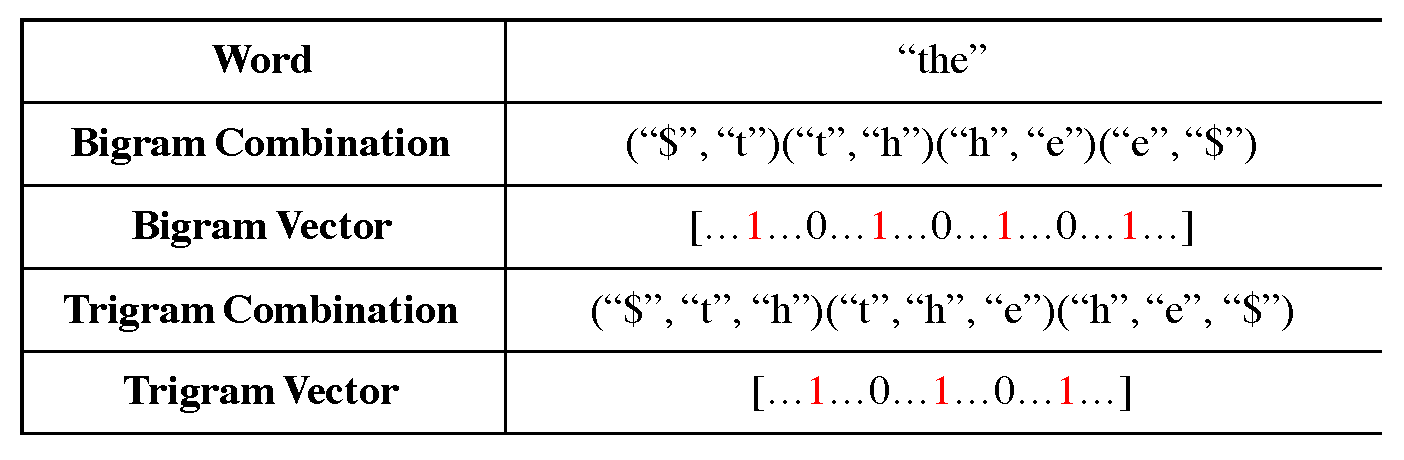
\epsfig{file=pic/bitri.eps, width=0.9\columnwidth}
%	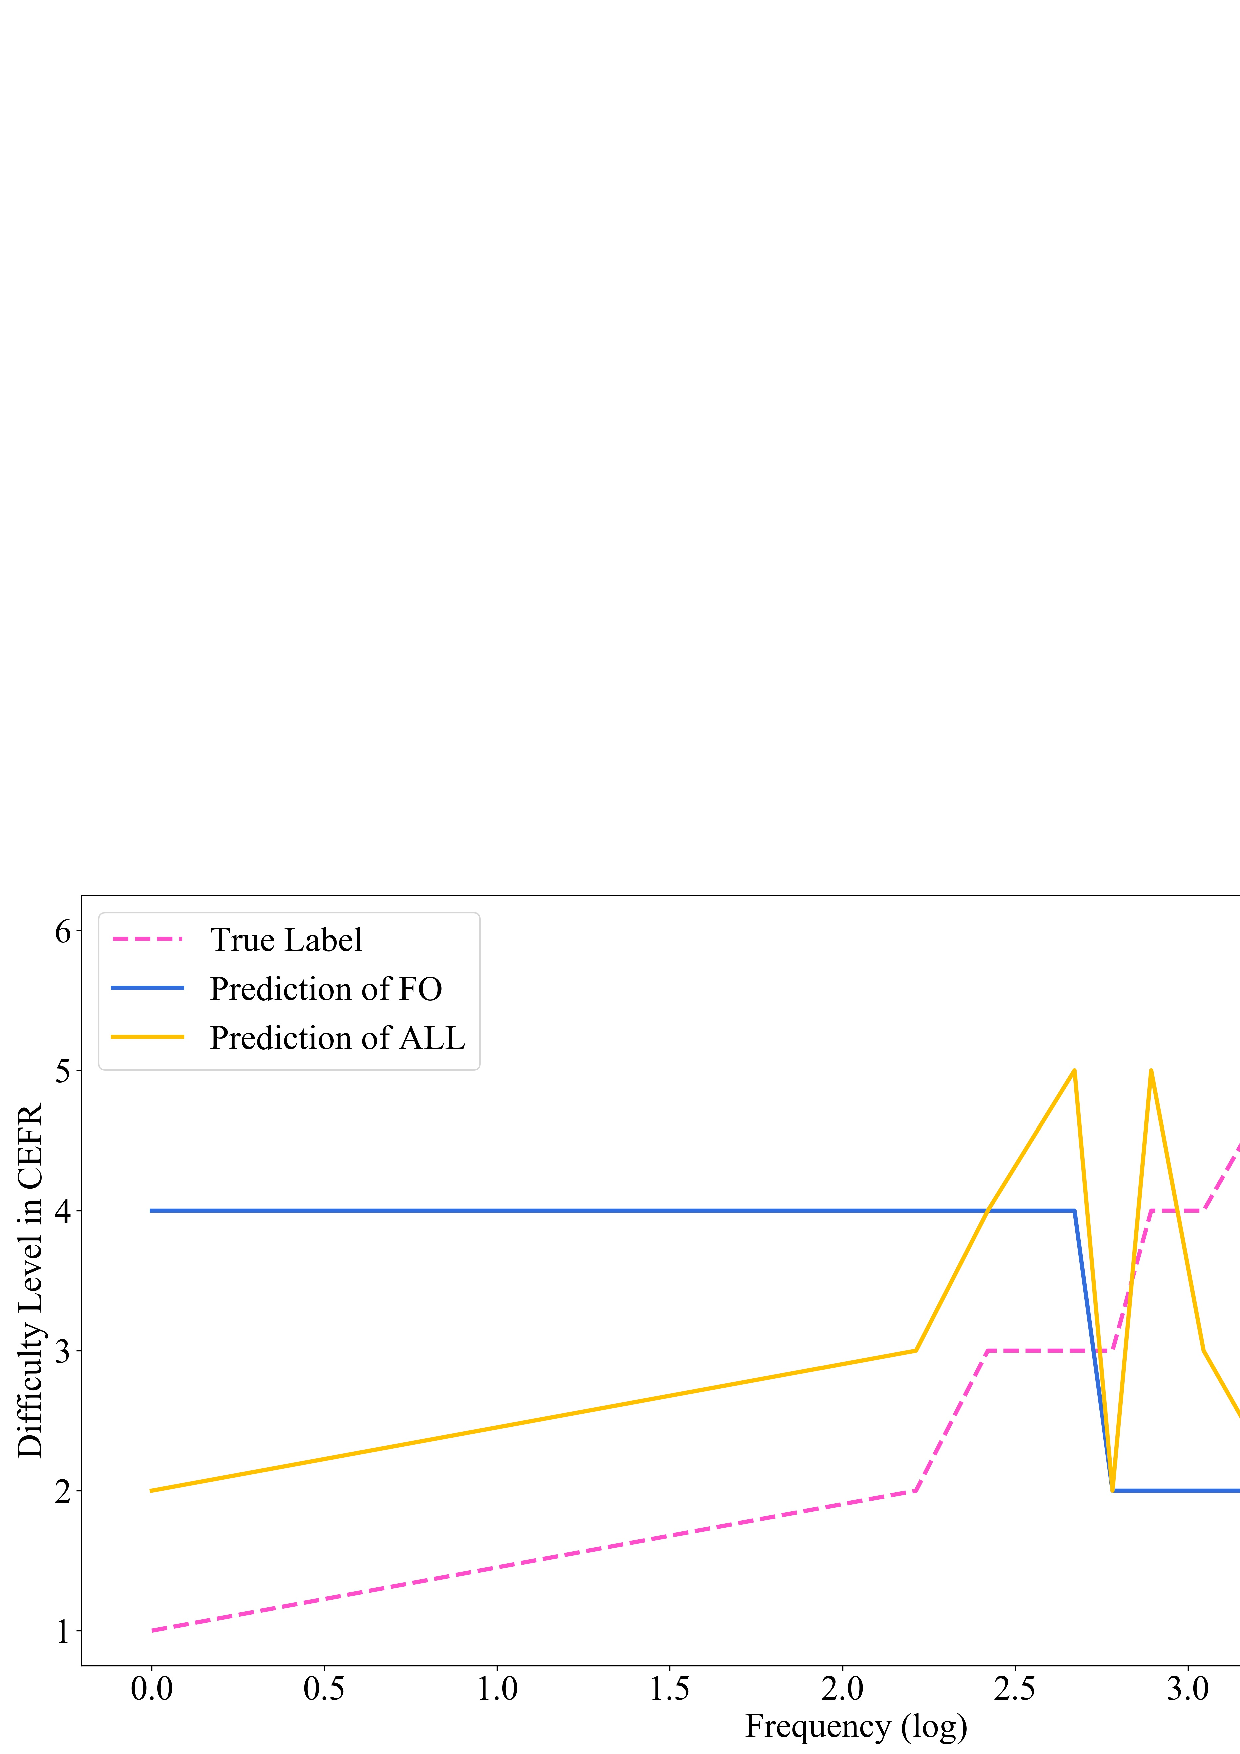
\includegraphics[width=0.5\linewidth]{pic/distance.pdf} 
%	\caption{The relation between log frequency and CEFR levels.
%					Lines show the distance between ground truth and wrongly predictions by FO and Fix+Word2Vec.}
%	\label{fig:distance}
%\end{figure}
%The above results show the prediction of our multi-faceted model (Fix+Word2Vec) is more closer to the ground truth.
%The correlation coefficients in Table \ref{tab:coefficients} also indicates our predictions have a certain correlation with the ground truth compared with baseline model FO.
%\begin{table}[th]
%	\centering
%	\scriptsize
%	\begin{tabular}{|c|c|c|}
%		\hline
%		& \textbf{Pearson} & \textbf{Spearman} \\ \hline
%		\textbf{Ground Truth\&FO} & -0.057 & -0.092 \\ \hline
%		\textbf{Ground Truth\&Fix+Word2Vec} & 0.305 & 0.300 \\ \hline
%	\end{tabular}
%	\caption{\label{tab:coefficients} Correlation coefficient table.}
%\end{table}

%The average accuracy of human classification evaluation is 49.28  for English and 44.44  for German.
%As for difficulty ranking task, the average accuracy of human evaluation is 88.89  for English and 65.85  for German.
%%For English, the accuracy of human labeling is 49.28  and for German, there is an accuracy of 44.44 .
%%That is to say, human can get the correct difficulty level of words with a chance of over 45 . As a result, our work is meaningful because it proves that people can't get a high accuracy by understanding the difficulty level of words in a short time.
%That is to say, it is a truly difficult task that even human can not achieve high accuracy given limited training. 
%In this way, our model 
%which achieves an accuracy around 45 on classification task and 75 on ranking task for both languages is considered very strong.
%Specifically, in English, the accuracy on classification and ranking tasks is close to human behavior.
%In German, the performance of our multi-faceted features is better than human.
%%This result indicates that figuring out the difficulty levels manually with a short-time training is a truly difficult task. 
%%In English, the classification results of multi-faceted are very close to human accuracy. 
%That is to say, our work is once again shown to be meaningful and there is still room for improvement.
%\SY{+Chinese}

\SY{Comparing both the classification and ranking results with human baseline, it is observed that}

\subsection{Ablation Test and Feature Selection}
% and Robustness in Different Corpora
\label{sec:embedding}
Based on the extracted features, we use the multi-layer perceptron (MLP) to investigate the effectiveness of each single feature and their combination MFF.
%We denote the combination of all the features as ALL.
%Then the performance of each individual feature is measured by removing it from MFF one at a time.

\begin{table}[ht]
	\scriptsize
	\setlength{\abovecaptionskip}{0pt}
	\setlength{\belowcaptionskip}{0pt}
	\begin{center}
		\begin{tabular}{lcccc}
		\toprule[1pt]
		&\textbf{NY Times} & \textbf{Gutenberg} & \textbf{German} & \textbf{Chinese} \\ 
		\midrule
	\textbf{MFF}&     \textbf{42.94 }       &   \textbf{41.18 }   &\textbf{47.74 }     &    \textbf{56.96} \\ 
	\midrule
		\textbf{MFF-Freq}     &      40.81     &     40.51 &      47.12      &  51.64  \\ 
	\textbf{MFF-Length}      &    41.72  &  40.90       &  43.00       &  52.36 \\ 
	\textbf{MFF-Phoneme}   &       42.32         &   40.14     &      41.98       &   54.96    \\ 
	\textbf{MFF-BiVec}    &        42.85   &40.77 &       43.00     &    56.70   \\ 
		\textbf{MFF-TriVec}   &         41.28  &   41.11   &46.71     &    55.92   \\ 
	\textbf{MFF-BiProb}    &          42.04     &       38.98   &      45.06        &   56.10  \\ 
		\textbf{MFF-TriProb}  &    41.46         &	39.61       &       45.88      &  52.42   \\ 
	\textbf{MFF-POS}      &      40.70      &      40.93   &       43.21   & 55.32 \\ 
	\textbf{MFF-Dependency}&     38.65               &  37.52   &      46.71      &   55.20    \\ 
		\textbf{MFF-Embedding} &34.22                  & 33.78      & 41.36     &   45.16  \\ 
		\bottomrule[1pt]
	\end{tabular}
	\end{center}
\caption{\label{tab:featurecompare} Classification ablation test of accuracy with each individual feature taken away. 
	Accuracy shown is the average of ten runs. The embedding in this table is Word2Vec.}
\end{table}

Table \ref{tab:featurecompare} shows the classification results of MFF
% and the different compounds with each individual feature taken away.
and each individual feature which are measured by removing it from MFF one at a time,
%In this table, we use Word2Vec to get the word embeddings.
%\SY{Do we need to mention the other embeddings?}
%, because it has a better performance than the other two embeddings which will be shown in the Appendix.
then we find MFF has the best performance.
The lower accuracy of a compound with certain individual feature taken away, the more effective this feature is.
%The most effective features are bolded in all columns.
Then it is observed that 
%We have once again confirmed that 
word frequency is not the determining factor for word difficulty.
% and this phenomenon is more pronounced in German.
%Under both English corpora, the embedding and dependency are top-two effective features.
%While in German, although embedding is still the best feature, we find that the intra-word features of words have a competitive performance.
%\SY{Chinese}
For English, German and Chinese, word embedding is most effective for word difficulty,
while other features behave differently in different languages.
%To show the correctness of the above discovery, 
To investigate the effectiveness of  features under different languages, 
we intuitively conduct the experiments on combination of features in different aspects, 
and the results are in Table \ref{tab:featureL}.

\begin{table}[ht]
	\scriptsize
	\setlength{\abovecaptionskip}{0pt}
	\setlength{\belowcaptionskip}{0pt}
	\begin{center}
		\begin{tabular}{lcccc}
		\toprule[1pt]
		\textbf{}            & \textbf{NY Times}& \textbf{Gutenberg} & \textbf{German} & \textbf{Chinese} \\
		\midrule
		\textbf{MFF}       &      \textbf{42.94}       &   \textbf{41.18}   &\textbf{47.74}    & \textbf{56.96}  \\
		\midrule
		\textbf{Frequency+Length} &      34.13        &      29.55        &      36.05    & \textbf{55.54}  \\ 
		\textbf{Intra-word Features} &      28.14        &      28.45        &      \textbf{44.32}     & 41.82  \\ 
		\textbf{Syntactic Features}     &      31.51        &      30.56        &      39.34    &   52.28  \\ 
		\textbf{Semantic Feature}       &      \textbf{39.40}       &      \textbf{36.82}       &      37.82     & 52.40   \\ 
		\bottomrule[1pt]
	\end{tabular}
	\end{center}
\caption{\label{tab:featureL} Comparison of classification accuracy on different feature aspects on three languages.
Each accuracy is the average of ten runs. The embedding in this table is Word2Vec.}
\end{table}
 
This experiment makes an discovery that intra-word features play a very important role in German words, 
%even though in English it doesn't seem to be as important as other features. 
then frequency and length plays an important role in Chinese words.
%One reasonable explanation is that the pronunciation of German words is closely related to its difficulty which can be 
%discovered in Table \ref{tab:featurecompare} and German words are usually 
%longer than English ones. \SY{+Chinese}
One reasonable explanation is that the pronunciation of German words is closely related to its difficulty which can be 
discovered in Table \ref{tab:featurecompare}.
For Chinese, the construction of HSK vocabulary fully considers the role of frequency.
In addition, it shows that the length of words increases with difficulty level, following the statistical mapping 
\{H1: 1.50, H2: 1.64, H3: 1.78, H4: 1.86, H5: 1.89, H6: 2.04\}.
For English, 
comparing the features extracted from NY Times and Gutenberg, the relative strength of different feature aspects are similar, suggesting strong robustness of the model against different environments.

%According to the results in Table \ref{tab:featurecompare}, word embedding extracted by Word2Vec is the strongest feature to identify word difficulty, so we will consider the effectiveness of  other word embedding models in later contrast experiments on classification and word-pair ranking tasks.

The results in Table \ref{tab:featurecompare} and \ref{tab:featureL} shows the obvious advantages of word embeddings, 
then we design experiments to investigate the performance of different embeddings.
Table \ref{tab:embedding} is the classification result for MFF with different embeddings, such as Word2Vec, GloVe and BERT.
The best results appear between Word2Vec and BERT, but there is no obvious advantages on BERT.
%trend on BERT.
When analyzing the features of different embeddings, we will find that Word2Vec and GloVe combine all the different senses of word into one fixed vector. 
Different from the traditional word embedding algorithms, BERT model can capture the context of a word and clearly distinguish polysemy of a word in the sentence-level tasks.
However, when applying it to word level,  each word is represented with a fixed vector which mixes all the contextual information together and the advantage of BERT model has been defeated.
\begin{table}[ht]
	\scriptsize
	\setlength{\abovecaptionskip}{0pt}
		\setlength{\belowcaptionskip}{0pt}
	\begin{center}
		\begin{tabular}{lcccc}
		\toprule[1pt]
		\textbf{}            & \textbf{NY Times}& \textbf{Gutenberg} & \textbf{German} & \textbf{Chinese} \\
		\midrule
		\textbf{MFF[Word2Vec]} &   \textbf{42.94 } & 41.18  & \textbf{47.74 } &   \textbf{56.96}    \\ 
		\textbf{MFF[GloVe]} &    36.80  & 38.77  & 46.91  &   56.22   \\ 
		\textbf{MFF[BERT]}     &   42.11  & \textbf{41.76 } & 46.30  &  53.78   \\ 
		\bottomrule[1pt]
	\end{tabular}
	\end{center}
\caption{\label{tab:embedding} Classification results with the features including different embeddings.}
\end{table}

